%Results
\section{Descriptive statistics}
Before the experiment, the seeds were weighted in groups of ten, to see if there was a baseline difference between certain genotypes. Table \ref{tab:germination_percentage}, in the previous section, displays the measured weights.
After the completion of the experiment, the outliers were identified, and each plant was attributed a specific weight, following the protocol described in material and methods section. Those weights were used to compute the weighted mean and weighted standard deviation of the fresh and dry weight of the root system and the leaf system, as well as the area of the root system, for each plant. These results are presented in table \ref{tab:summary_table_all_variables}.

\begin{table}[ht]
\centering
\caption[Weighted mean and standard deviation for each genotype]{Weighted mean and standard deviation for each genotype. $\mathbf{DRY_{LS}}$ represents the dry weight of the leaf system; $\mathbf{DRY_{RS}}$, the dry weight for the root system; $\mathbf{FRESH_{LS}}$, the fresh weight for the leaf system and $\mathbf{FRESH_{RS}}$, the fresh weight for the root system. All the results are presented as mean $\pm$ standard deviation (g)}
\rowcolors{2}{gray!25}{white} 
\begin{tabular}{lrrrr}
  \toprule
Genotype & $DRY_{LS}$ & $DRY_{RS}$ & $FRESH_{LS}$ & $FRESH_{RS}$ \\ 
  \midrule
1 & 0.2267 $\pm$ 0.0869 & 0.2354 $\pm$ 0.0698 & 2.7231 $\pm$ 1.1612 & 3.4447 $\pm$ 1.4431 \\ 
  2 & 0.2113 $\pm$ 0.0993 & 0.1964 $\pm$ 0.06 & 2.4058 $\pm$ 1.254 & 2.2725 $\pm$ 1.1119 \\ 
  3 & 0.2132 $\pm$ 0.0747 & 0.1939 $\pm$ 0.0474 & 2.406 $\pm$ 1.0814 & 2.8146 $\pm$ 1.3663 \\ 
  4 & 0.227 $\pm$ 0.1148 & 0.1824 $\pm$ 0.0861 & 2.45 $\pm$ 1.5508 & 2.7773 $\pm$ 2.1926 \\ 
  5 & 0.2126 $\pm$ 0.113 & 0.1829 $\pm$ 0.0606 & 2.6521 $\pm$ 1.5044 & 3.0241 $\pm$ 1.7336 \\ 
  6 & 0.2024 $\pm$ 0.0739 & 0.1747 $\pm$ 0.051 & 2.4244 $\pm$ 1.1691 & 3.2168 $\pm$ 1.4545 \\ 
  7 & 0.126 $\pm$ 0.0441 & 0.1251 $\pm$ 0.0232 & 1.4118 $\pm$ 0.5677 & 1.5669 $\pm$ 0.5783 \\ 
  8 & 0.186 $\pm$ 0.0805 & 0.1798 $\pm$ 0.0567 & 2.3614 $\pm$ 1.1696 & 2.6894 $\pm$ 1.273 \\ 
  9 & 0.1559 $\pm$ 0.0865 & 0.2064 $\pm$ 0.0574 & 1.9704 $\pm$ 1.1782 & 2.3862 $\pm$ 1.3949 \\ 
  10 & 0.1885 $\pm$ 0.0875 & 0.1769 $\pm$ 0.0693 & 2.1228 $\pm$ 1.046 & 2.029 $\pm$ 1.0451 \\ 
  11 & 0.1789 $\pm$ 0.0811 & 0.1783 $\pm$ 0.0521 & 2.1608 $\pm$ 1.0747 & 2.339 $\pm$ 1.2172 \\ 
  12 & 0.1684 $\pm$ 0.0893 & 0.1469 $\pm$ 0.0417 & 2.0166 $\pm$ 0.9281 & 2.0985 $\pm$ 0.9015 \\ 
  13 & 0.1927 $\pm$ 0.0794 & 0.1639 $\pm$ 0.054 & 2.1326 $\pm$ 1.077 & 2.1176 $\pm$ 1.1582 \\ 
  14 & 0.2438 $\pm$ 0.1288 & 0.2173 $\pm$ 0.0796 & 3.0901 $\pm$ 1.6735 & 3.486 $\pm$ 1.8646 \\ 
  15 & 0.1175 $\pm$ 0.0885 & 0.2097 $\pm$ 0.0591 & 1.48 $\pm$ 1.2962 & 1.8417 $\pm$ 1.3372 \\ 
  16 & 0.3244 $\pm$ 0.1276 & 0.2208 $\pm$ 0.0879 & 3.7094 $\pm$ 1.8196 & 3.9028 $\pm$ 2.2598 \\ 
  17 & 0.2357 $\pm$ 0.1111 & 0.2019 $\pm$ 0.065 & 2.7519 $\pm$ 1.2418 & 2.8555 $\pm$ 1.4 \\ 
  18 & 0.1427 $\pm$ 0.039 & 0.1653 $\pm$ 0.0442 & 1.5621 $\pm$ 0.5627 & 1.7781 $\pm$ 0.8075 \\ 
  19 & 0.1785 $\pm$ 0.0505 & 0.1926 $\pm$ 0.04 & 2.0917 $\pm$ 0.7454 & 2.7726 $\pm$ 0.9668 \\ 
  20 & 0.1901 $\pm$ 0.0721 & 0.1506 $\pm$ 0.0497 & 2.0641 $\pm$ 0.9693 & 2.2429 $\pm$ 1.2908 \\ 
  21 & 0.1649 $\pm$ 0.0786 & 0.1859 $\pm$ 0.0329 & 1.9682 $\pm$ 0.8601 & 1.7689 $\pm$ 0.6407 \\ 
  22 & 0.1482 $\pm$ 0.0669 & 0.1508 $\pm$ 0.0296 & 1.522 $\pm$ 0.7799 & 1.793 $\pm$ 0.838 \\ 
  23 & 0.156 $\pm$ 0.04 & 0.1574 $\pm$ 0.0372 & 1.7621 $\pm$ 0.6537 & 1.9874 $\pm$ 0.9962 \\ 
  24 & 0.1668 $\pm$ 0.0827 & 0.1236 $\pm$ 0.0575 & 1.9357 $\pm$ 0.8693 & 2.0506 $\pm$ 1.2218 \\ 
  25 & 0.2013 $\pm$ 0.0856 & 0.1195 $\pm$ 0.0481 & 2.4338 $\pm$ 1.0937 & 1.9605 $\pm$ 1.1428 \\ 
  26 & 0.1463 $\pm$ 0.075 & 0.1573 $\pm$ 0.0365 & 1.7995 $\pm$ 1.1967 & 1.9256 $\pm$ 1.0053 \\ 
  27 & 0.1682 $\pm$ 0.0894 & 0.188 $\pm$ 0.0401 & 2.2662 $\pm$ 1.0855 & 2.3647 $\pm$ 1.0382 \\ 
  28 & 0.1753 $\pm$ 0.0865 & 0.2244 $\pm$ 0.066 & 2.0357 $\pm$ 1.0699 & 2.441 $\pm$ 1.1785 \\ 
  29 & 0.215 $\pm$ 0.0934 & 0.1823 $\pm$ 0.0663 & 2.4861 $\pm$ 1.3776 & 2.6743 $\pm$ 1.5787 \\ 
  30 & 0.1573 $\pm$ 0.0592 & 0.184 $\pm$ 0.0485 & 2.1033 $\pm$ 0.8712 & 2.51 $\pm$ 1.1265 \\ 
   \bottomrule
\end{tabular}
\label{tab:summary_table_all_variables}
\end{table}

\begin{figure}
\centering
	\begin{subfigure}[t]{\textwidth}
		\centering
		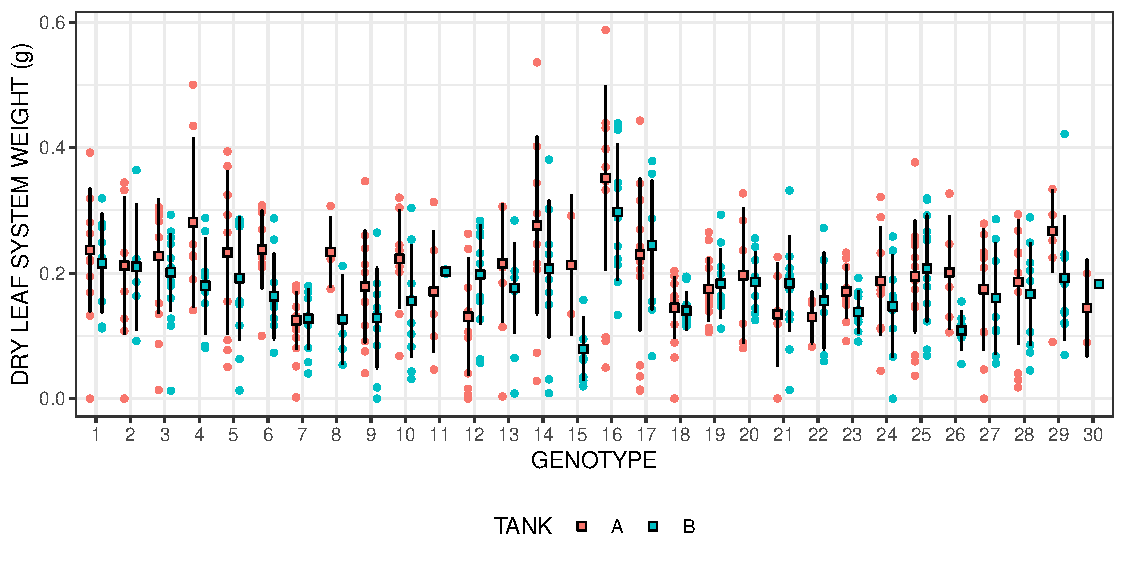
\includegraphics[width = \textwidth]{../../Figures/DRY_LS_summary_plot.pdf}
		\caption{Dry leaf weight ($DRY\_LS$)}
	\end{subfigure}

	\begin{subfigure}[t]{\textwidth}
		\centering
		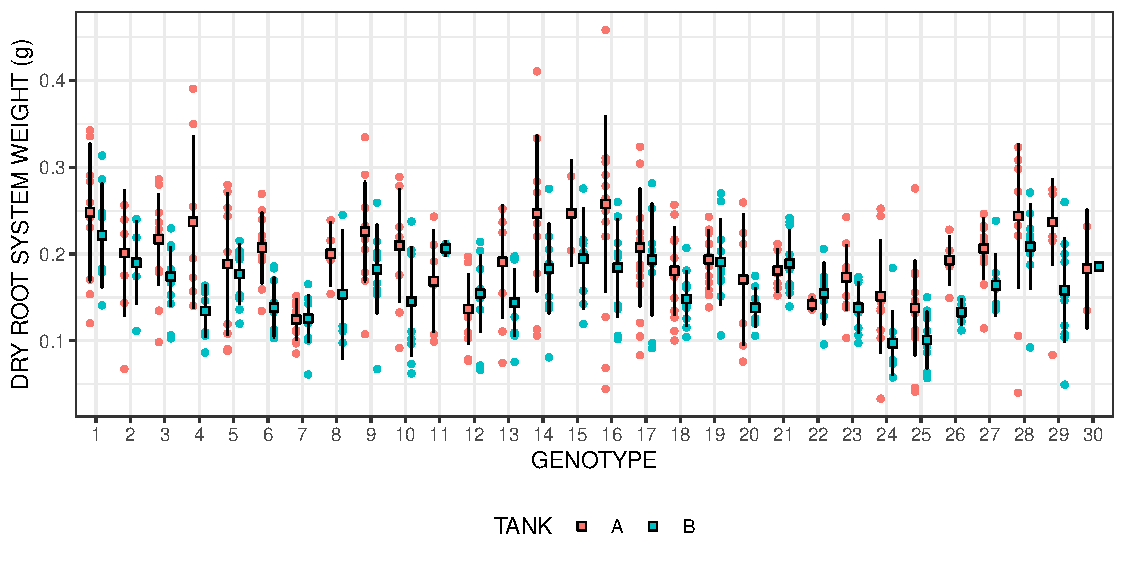
\includegraphics[width = \textwidth]{../../Figures/DRY_RS_summary_plot.pdf}
		\caption{Dry root weight ($DRY\_RS$)}
	\end{subfigure}
	\caption{Dotplot displaying mean weight (\protect\emptysquare) and associated standard deviation (\protect\blackline), grouped by tanks for each variable.}
\end{figure}
\begin{figure}\ContinuedFloat
	\begin{subfigure}[t]{\textwidth}
		\centering
		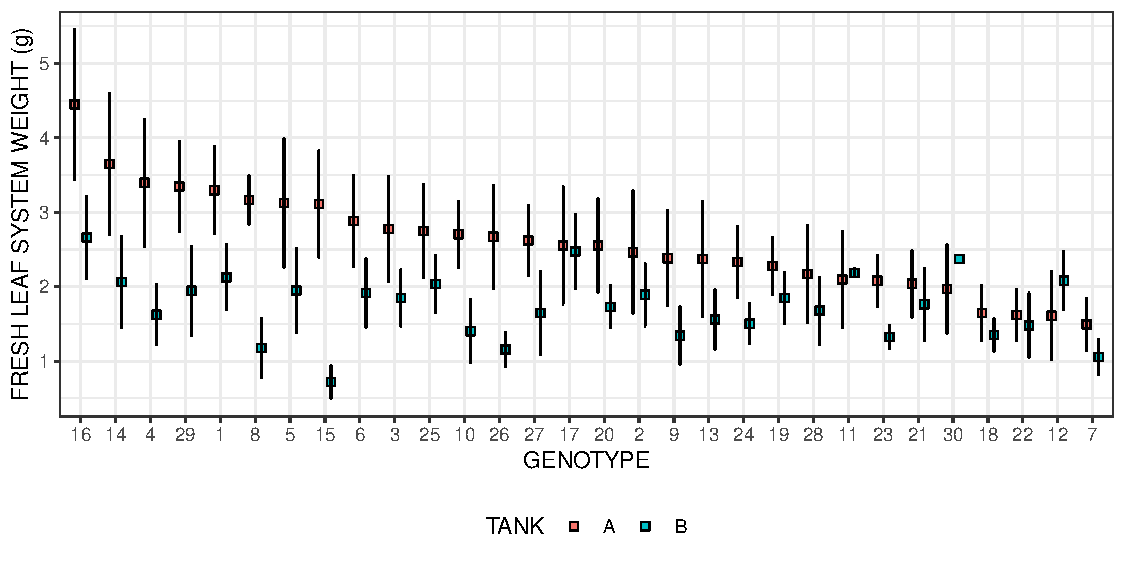
\includegraphics[width = \textwidth]{../../Figures/FRESH_LS_summary_plot.pdf}
		\caption{Fresh leaf weight ($FRESH\_LS$)}
	\end{subfigure}

	\begin{subfigure}[t]{\textwidth}
		\centering
		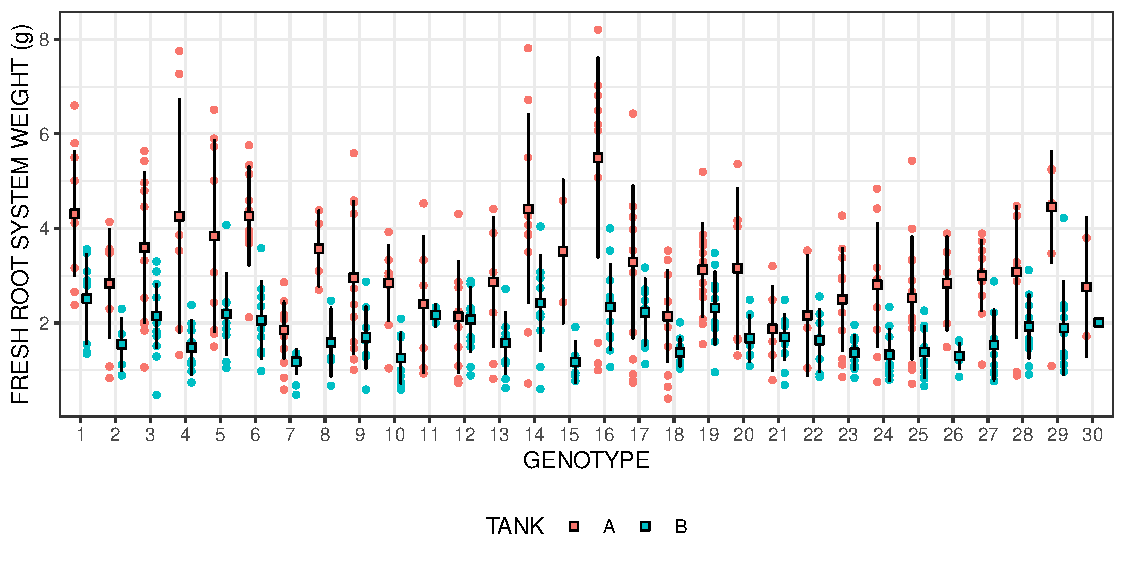
\includegraphics[width = \textwidth]{../../Figures/FRESH_RS_summary_plot.pdf}
		\caption{Fresh root weight ($FRESH\_RS$)}
	\end{subfigure}
	\caption{Dotplot displaying mean weight (\protect\emptysquare) and associated standard deviation (\protect\blackline), grouped by tanks for each variable.}
\end{figure}

\section{SpATS analysis}
\section{ARxAR model analysis}
\section{Model comparison}
\subsection{Performances}
\subsection{Parametrization}
\subsection{Modelling strategy}
